\label{ArchitekturundVerhalten}

%\begin{figure}[!hbt]
%	\centering
%	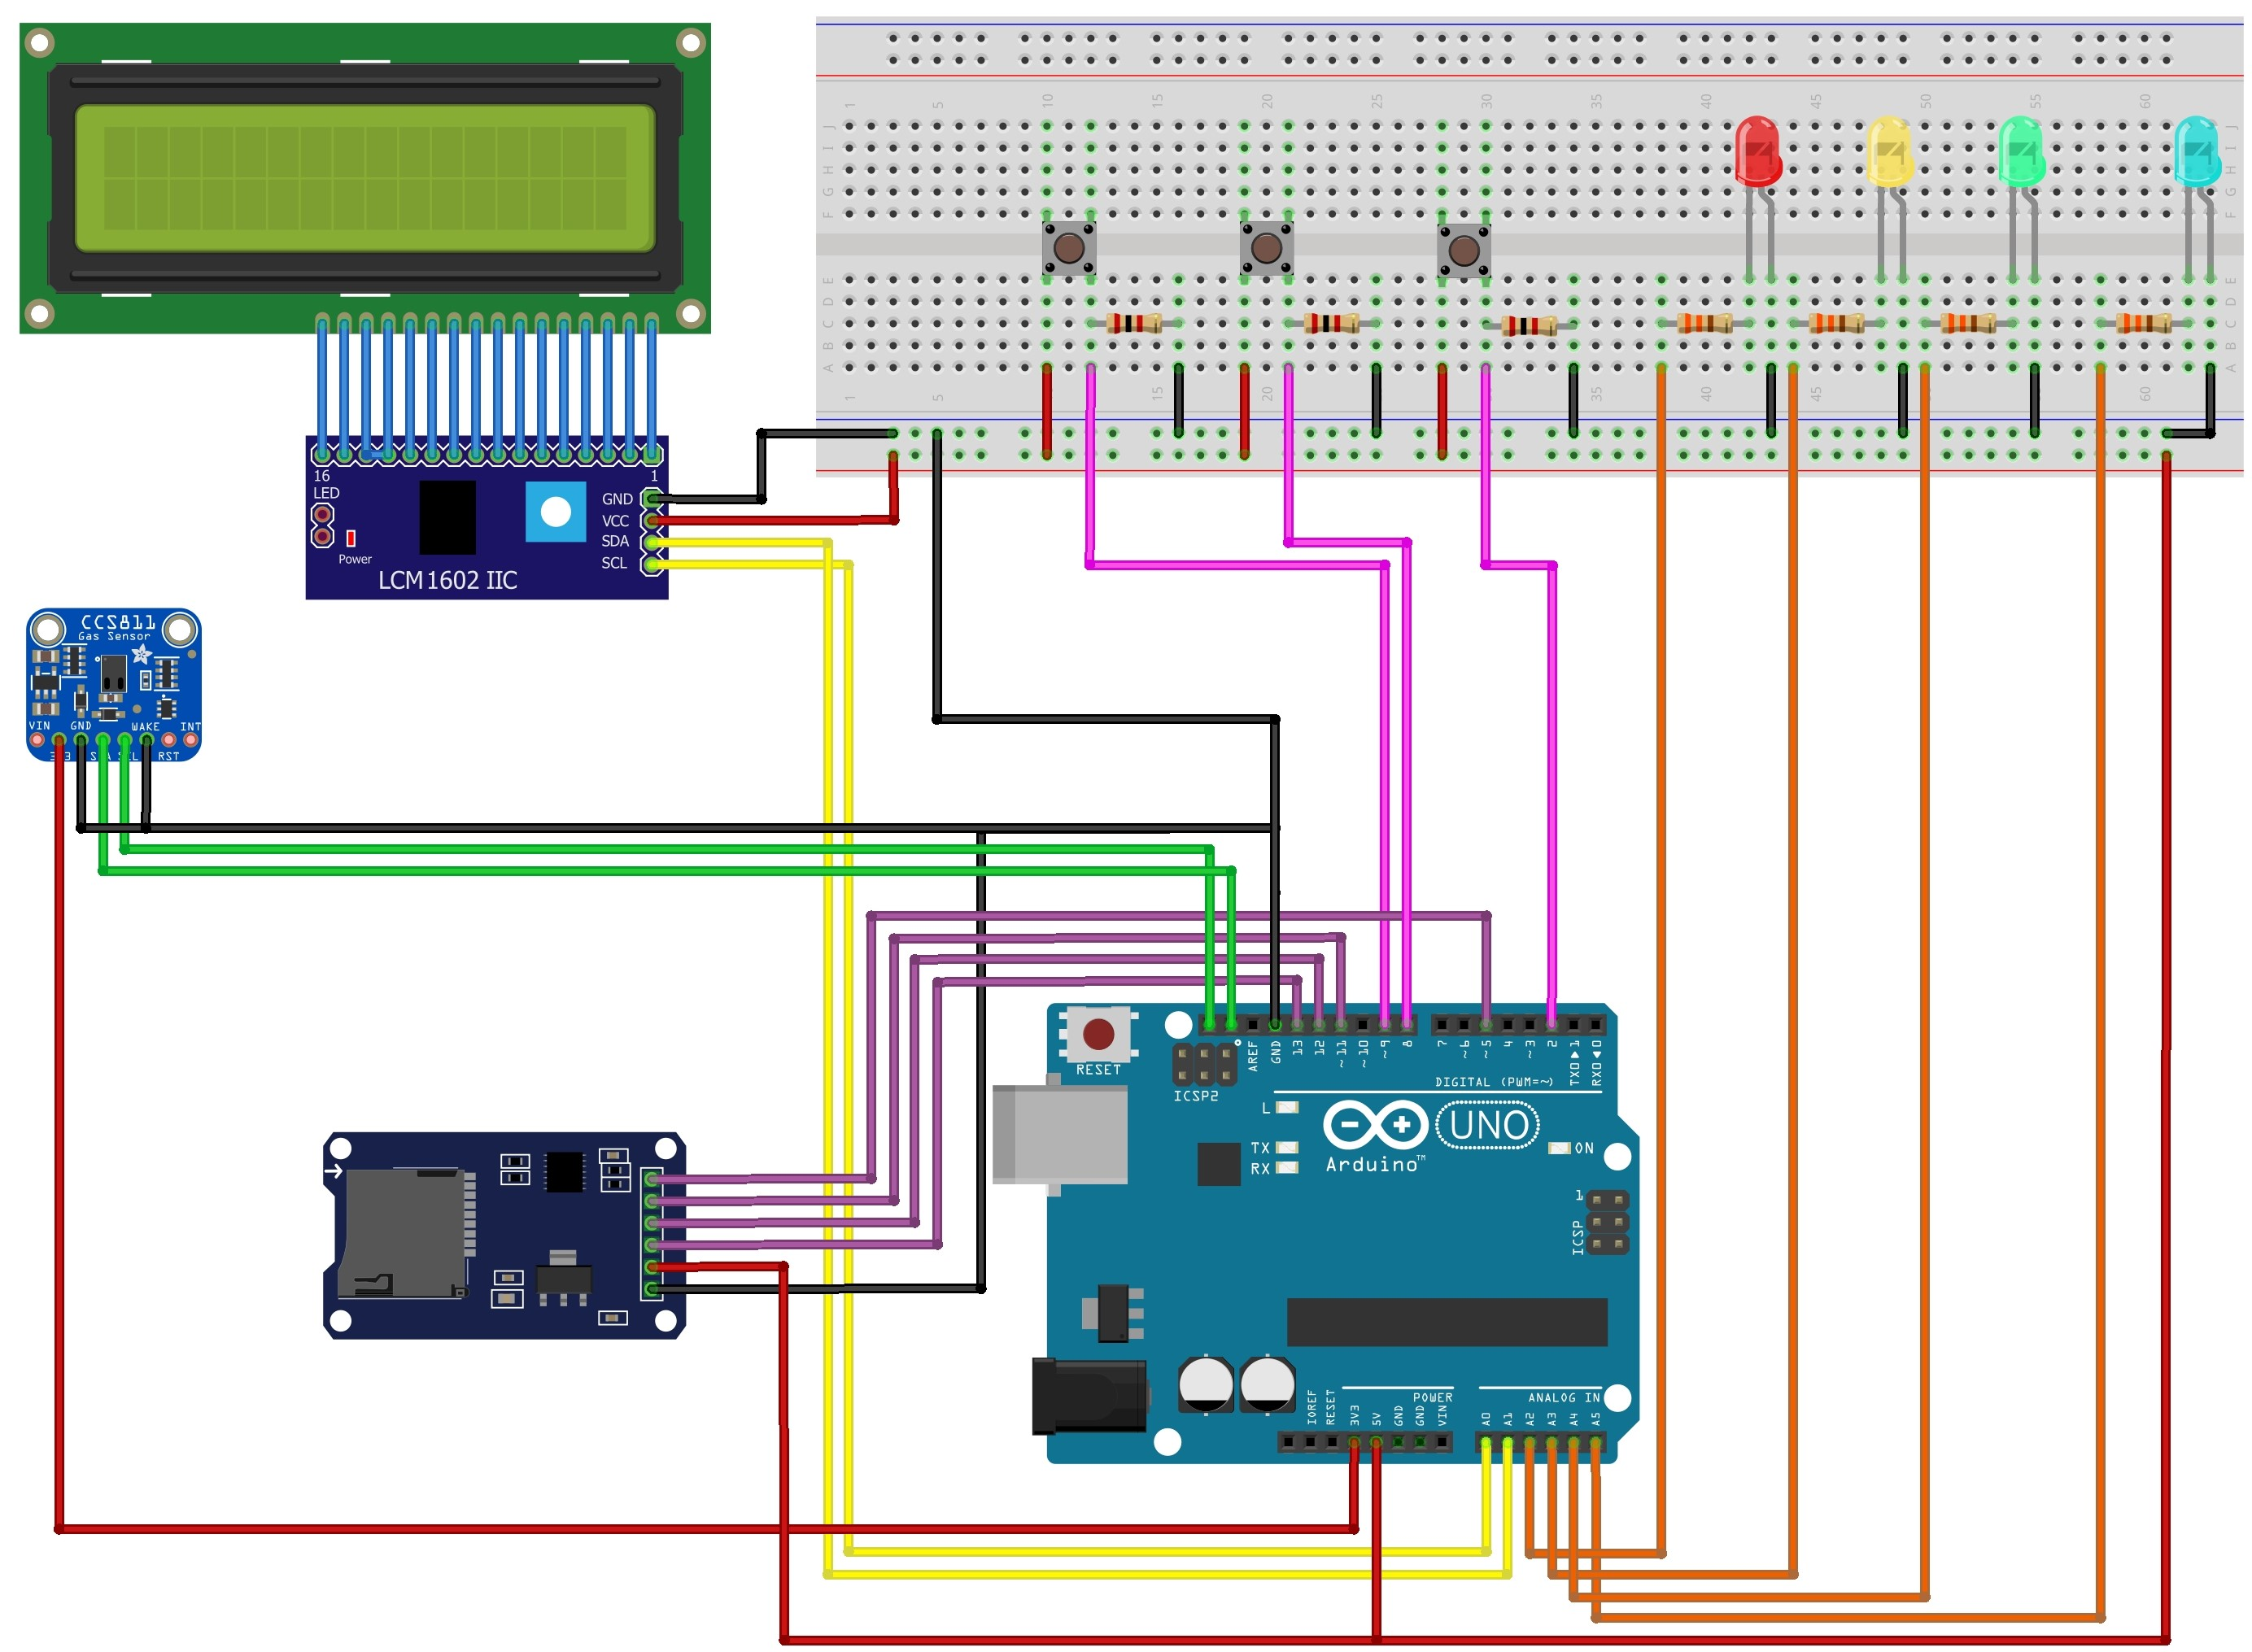
\includegraphics[width=0.9\linewidth]{Images/Layout_Steckplatine}
%	\caption{Entwurf der Toplevel-Architektur mithilfe von Enterprise Architect}
%	\label{fig:ToplevelArchitektur}
%\end{figure}

Damit der genaue Ablauf unseres Programms definiert ist, wurde mithilfe von Enterprise Architect ein Zustandsdiagramm erstellt. \\
Dieses Diagramm ist dazu da, die Zustände, in welches sich das Objekt befindet, zu präsentieren. Auch die Übergänge zwischen den einzelnen Zuständen wird hier deutlich. Zudem zeigt es den Anfangs- und Endpunkt einer Sequenz von Zustandsänderungen. \cite[vgl. S. 120]{JosephSchmuller.2000} \\
Auf unser Projekt übertragen bedeutet es, dass das Diagramm vom Einschalten der Hardware, durch Stromversorgung des Arduinos, über jede Kombinationsmöglichkeiten der Taster, bis hin zum wieder Ausschalten der Hardware, alle Zustände zeigt, in welche das Programm kommen kann. Dies soll später dem Softwareentwickler die Arbeit vereinfachen. Des Weiteren können auch Tests mithilfe des Zustandsdiagramms leichter durchgeführt werden, da die Eingangsvariablen mit den darauffolgenden Zustandsänderungen, wie in \ref{fig:Statemachine}, eindeutig zu erkennen sind. \\

\begin{figure}[!hbt]
	\centering
	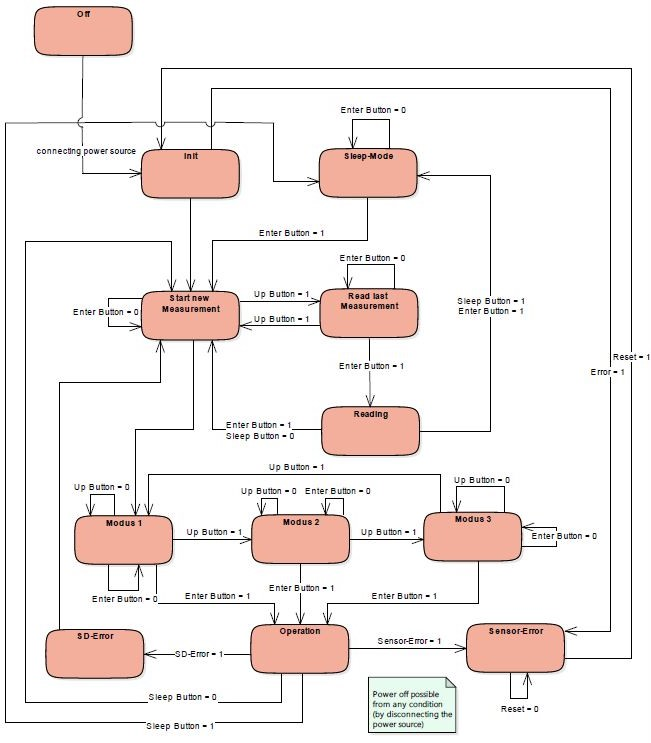
\includegraphics[width=0.9\linewidth]{Images/Statemachine}
	\caption{Entwurf des Zustandsdiagramms mithilfe von Enterprise Architect}
	\label{fig:Statemachine}
\end{figure}

Das Komponentendiagramm, welches in \ref{fig:KomponentenDiagramm} zu sehen ist, soll dazu dienen, alle Aktoren und deren Verbindungen darzustellen. \\

\begin{figure}[!hbt]
	\centering
	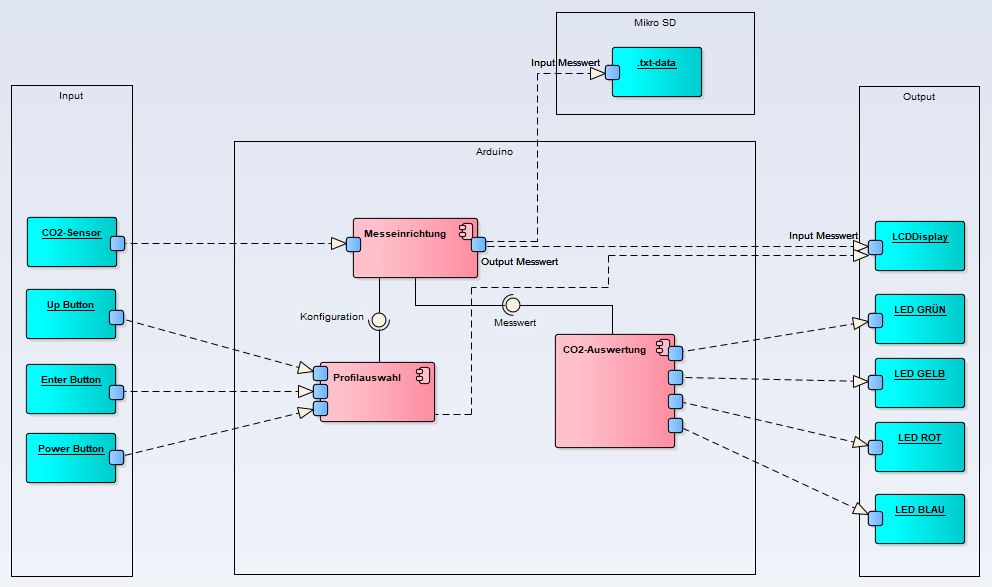
\includegraphics[width=0.9\linewidth]{Images/Komponentendiagramm}
	\caption{Entwurf des Komponentendiagramms mithilfe von Enterprise Architect}
	\label{fig:KomponentenDiagramm}
\end{figure}